\chapter{\label{design}Design}
We have seen, that the current bitcoin client does not scale well because of its inter-thread communication. While there are different approaches to speed up or eliminate inter-thread communication, we propose a different solution to the problem. We reduce the tasks of the relay to the bare minimum. The sole purpose of the new client should be to relay blocks. We propose to have a special programmable switch which acts as a block cache. A special firmware is able to translate requests into local lookups. A separate controller hosts the more sophisticated part of the logic, like validating blocks. This controller is responsible for updating the switch with new blocks upon their arrival and informs connected peers about the new block. The design uses UDP as the underlaying transport protocol. The benefit of this is, that due to its stateless nature, a UDP based protocol is able to scale better. As much work as possible is handled in hardware. This framework is called SABRE and is the design of M.Apostolaki and the Networked Systems Group at ETH Zürich \cite{apostolaki2018}.\\
We solve all scaling problems of the current bitcoin client noted in chapter \ref{profiling}: Only one client is effectively connected to the controller at a given time. Therefore, we see from the measurements in chapter \ref{profiling} that we do not expect a large communication overhead. All other clients are able to request the blocks at line rate from the switch. Because the switch has a clearly defined response to a request, there is no need for inter-thread communication. Therefore, there is no scaling problem of the inter-thread communication at the switch as well. The controller is able to handle multiple thousands simultaneous connections while using only one single socket for the connection to the switch. This solves the limited socket problem that is imposed by the use of FD\_SET. As we will show in the evaluation in chapter \ref{evaluation}, the design also uses considerably less memory per connection.\\
This thesis focuses on the modifications that are necessary on the clients and the controller. In this chapter, the message protocol is presented in \ref{sec:functional_overview}. The design of the client and the controller is presented in sections \ref{sec:design:design}. The chapter is concluded with a discussion of the shortcomings of the current design in section \ref{sec:design:shortcomings}.


\section{Terminology}
The design in this chapter and the following evaluation in chapter \ref{evaluation} use 3 different bitcoin clients. To avoid misconceptions, they are briefly explained here. For a more throughout explanation of the modified clients, see sections \ref{design:modifiedBitcoinClient} and \ref{design:SwitchController}. Also, a few other commonly used terms are defined here.
\subsubsection{Regular Bitcoin Client}
The term \textit{bitcoin client} is used for the unmodified bitcoin client from the official repository on GitHub \cite{bitcoinRepo}. Version 0.16 (commit bf3353de90598f08a68d966c50b57ceaeb5b5d96) was used throughout this work. We use the term \textit{regular} when referring to the unmodified bitcoin client or the unmodified bitcoin protocol.
\subsubsection{Modified Bitcoin Client}
The \textit{modified bitcoin client} is based on the \textit{bitcoin client} and is augmented with additional features. This allows the modified bitcoin client to connect to the switch relay. The modified bitcoin client can be used as a drop-in replacement for the bitcoin client.
\subsubsection{Controller}
The \textit{controller} is based on the \textit{bitcoin client} and is augmented with additional features. It is used to interface with the p4 switch and to modify its state. This code is not intended to run on a regular bitcoin node.
\subsubsection{Network protocol}
We refer to the regular bitcoin peer-to-peer network as the \textit{network protocol}. 
\subsubsection{Relay protocol}
We name the here presented addition to the communication logic \textit{relay protocol}, as it differs completely from the \textit{network protocol}.




\begin{figure}[bt]
  \begin{center}
	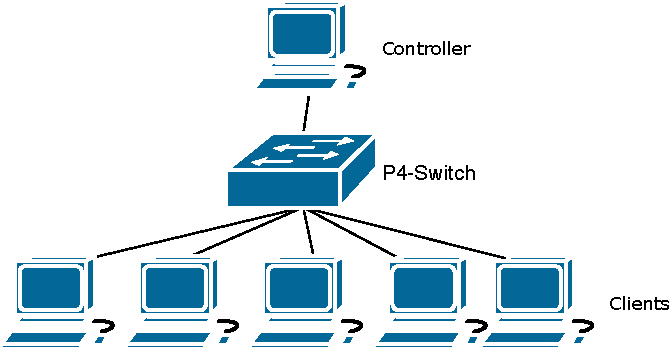
\includegraphics[width=0.5\textwidth]{Figures/DesignOverview}
  \caption{Overview of the different participants of the relay protocol.}
  \label{fig:setup:overview}
  \end{center}
\end{figure}

\section{Protocol overview \label{sec:functional_overview}}
The protocol that is presented here, differentiates among 3 parties. An overview can be found in figure \ref{fig:setup:overview}. The first group consists of the clients. We assume there to be many clients. The clients have 2 goals. They want to receive new blocks and they want to redistribute blocks that they have learned about. The second group consists of the switch. The switch is a piece of programmable hardware. It acts as a cache. Answers to a predefined set of requests can be delivered at line rate. The last protocol participant is the \textit{controller}. The \textit{controller} is used to handle uncacheable requests and to do the more sophisticated computation. It is also responsible for writing the data to the switch.\\
The protocol that connects these 3 groups is now presented. The design of the system and the network was done by M.Apostolaki and the Networked Systems group at ETH Zürich.\\
The protocol can roughly be split into 3 parts which are illustrated in figure \ref{figure:messagingProtocol}. Unless otherwise stated, UDP datagrams are used as underlaying transport protocol. The first part of the protocol (see figure \ref{figure:handshake}) handles the connection setup between the client and the switch. A 3-way handshake is used to establish the connection. The client initiates a handshake. After receiving the handshake request, the switch replies with a message containing a secret value. To complete the handshake, the client sends another message containing the same secret back to the switch. The secret is used to protect the switch from spoofing. After the handshake is complete, a message containing the connection details of the client is sent to the controller to store this metadata.\\
The second part of the protocol (figure \ref{figure:upd}) handles the update process of the switch. When a \textit{modified bitcoin client}, which is connected to the switch, receives a new block, it advertises it to the switch. If the switch does not know this block, it will tell the client to connect to the controller at a specified port/IP. This connection is established using the regular bitcoin protocol. After the client has connected to the controller, it will send the new block to the controller. After that, the connection is closed and the controller updates the switch. It will first send a message indicating, that a new block will be sent. After that, the block is sent in chunks of 499 bytes to the switch. These block fragments are called segments. The last segment is padded to have the same size. This is needed because of limitations of the switch. A precomputed UDP checksum is added, to reduce the computation that the switch has to do on an incoming request.\\
After the controller updated the switch, it will advertise the new block to all connected clients. Part 3 (figure \ref{figure:inv}) of the protocol explains how blocks are distributed to the clients. The controller sends an advertisement containing the hash of the block and the total number of segments, the block was split into. The clients that are interested in the block can request the individual segments from the switch directly. From this point on, the controller does not have to do any more work for distributing this block. A client has to request all segments seperately to be able to reconstruct the block.


\subsection{Message types \label{sec:messagingProtocol}}
The \textit{relay protocol} uses a set of message types for the communication between client, switch and controller. The message types and their use are listed here for reference. To see, in which part of the protocol the messages are used, see figure \ref{figure:messagingProtocol} The focus lays on the functional aspects of the message types. The exact message structures and sizes are listed in appendix \ref{appendixMessagingProtocol}. For better readability, the message types of the \textit{relay protocol} are written using capital letters throughout this thesis.
\begin{itemize}
	\item REY: This message type is used to establish a connection between the client and the switch. A 3-way handshake is performed. The messages of the individual steps of this handshake are marked using a flag.
	\item INV: The INV message is used by the controller to advertise new blocks. It contains the block hash and the number of segments the block is split into.
	\item SEG: Using the SEG message, the client requests a segment of a block from the switch. For this, the message contains the hash of the block and the segment number that is requested.
	\item BLK: The BLK message is used by the controller to update the switch. The message contains the segment ID and the data. Additionally, the packet contains a precomputed checksum which is used by the switch to create the UDP checksum when the client requests the block. Note that the UDP checksum depends on the destination port and can therefore not be computed in advance and must be calculated by the switch. \\ The switch sends BLK messages as reply to SEG messages from the client. These BLK messages only contain the segment ID and the data.
	\item ADV: The client sends an ADV message to the switch to indicate that it received a new block. This message contains the hash of the new block.
	\item CTR: The switch may respond to an ADV message with a CTR message, indicating that the client should connect to the controller. The message contains the IP and the port which should be used to connect to the controller.
	\item UPD: The UPD message is sent by the controller. The switch uses this message as an indicator, that the controller wants to add a new block. The message contains the hash of the new block.
	\item BCL: The BCL message is used to blacklist a peer and is sent from the client to the switch.
	\item CON: After a successful handshake with a new client, the switch sends a CON message with IP and port of the client to the controller. This message is used to inform the controller about new connections.
\end{itemize}




\begin{figure}[!bt]
\begin{center}
\begin{subfigure}[b]{0.32\textwidth}
	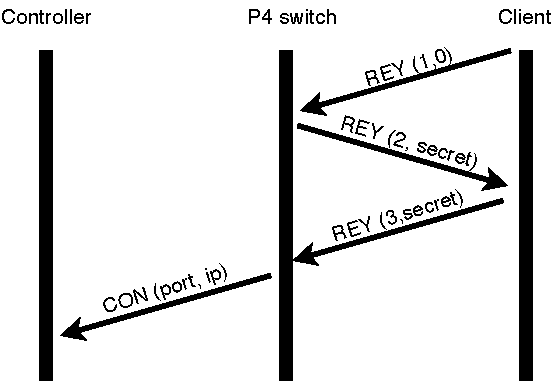
\includegraphics[width=\textwidth]{Figures/Handshake.pdf}
  \subcaption{Handshake}
  \label{figure:handshake}
\end{subfigure}
\begin{subfigure}[b]{0.32\textwidth}
	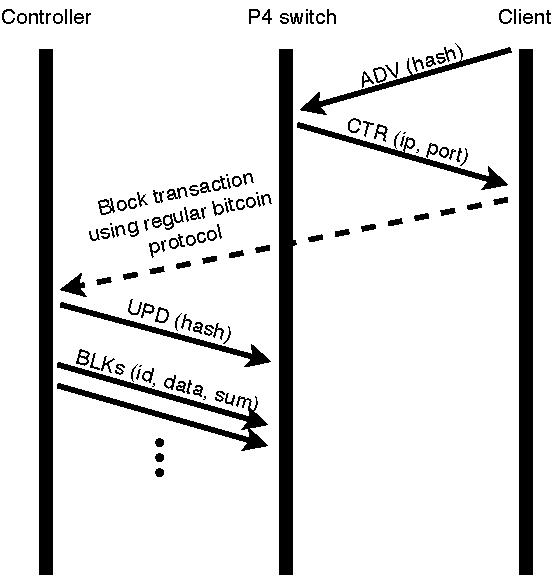
\includegraphics[width=\textwidth]{Figures/UPD.pdf}
  \subcaption{switch update}
  \label{figure:upd}
\end{subfigure}
\begin{subfigure}[b]{0.32\textwidth}
	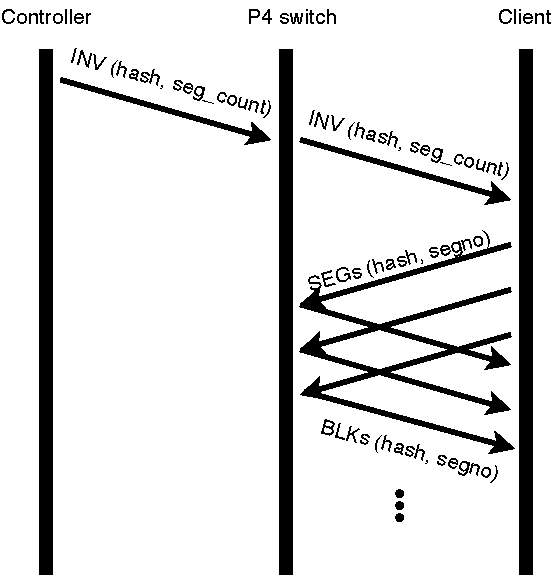
\includegraphics[width=\textwidth]{Figures/INV.pdf}
  \subcaption{client side block request}
  \label{figure:inv}
\end{subfigure}
\caption[Overview of the individual phases of the relay protocol.]{Overview of the individual phases of the \textit{relay protocol}.}
\label{figure:messagingProtocol}
\end{center}
\end{figure}




\section{Client and Controller Implementation  \label{sec:design:design}}
The changes to the bitcoin client aim at being lightweight and modular. First, we describe some general design choices that are common to both the \textit{modified client} and the \textit{controller}. Next, we discuss the peculiarities of the \textit{modified client} and the \textit{controller}.\\
The source of the implementation can be found in \cite{bitcoinFork}.

\subsection{General design}
Both, the \textit{modified client} and the \textit{controller} are based on the \textit{regular bitcoin client}. The benefit of this is, that parts of the existing code can be reused. One decision in the design process was to have most of the logic inside a separate C++ class to be able to quickly get an overview of the additional logic.\\
For better testability of the design, the 3 software types, namely the \textit{regular client}, the \textit{regular bitcoin client} and the \textit{controller} can be chosen at startup without the need to recompile. This results in a minimally larger binary compared to an approach where the type has to be specified at compile time. Besides the client type, other new command line or config file parameters were introduced. They allow to set the IP address and the port of the switch, as well as the own port that is used to connect to the relay. \\
Thanks to the socket abstraction, the logic for incoming messages can be reused. After a packet is read from the socket, the code checks if it is coming from the switch. If this is the case, it is handed over to the relay network message handler instead of the normal message handler. For sending, the handler checks if the outgoing message should use UDP before sending because the logic for sending is slightly different between TCP and UDP. Since UDP is connection-less the sender has to provide the destination IP and port.\\

\subsection{Modified Bitcoin Client \label{design:modifiedBitcoinClient}}
The modified client runs on a users device. Along the regular tasks of a regular bitcoin client, the modified client also fulfills the here mentioned tasks.
\subsubsection{Connection setup}
When the modified client starts its networking routine, a Net\_relay object is generated. This object is handles the logic that is used to interface with the switch. A new UDP port is created with the connection settings found in the settings. Using the command line or the config file, the default settings for ip address and port of the switch can be overwritten. In a productive setting, anycast could be used to find a relay switch. \\
The CNode construct of the unmodified bitcoin client was used to enhance the integration with the existing codebase. This allows, for example, to get a report over the connected switch using bitcoin-cli as it is possible with regular connections. To be able to differentiate between the UDP connection used for the switch and the TCP connections of regular peers, a isRelay flag was added to the CNode class.\\
After the CNode is created, the client tries to establish a connection to the switch. As long as the client is not connected to the switch, every minute, a handshake is initiated by sending a REY message. The switch will answer with another REY message containing a secret. Using the same secret, the 3-way handshake is concluded. After the handshake, the relay connection will go to a connected state which will activate all other switch specific functionalities.\\
The fact that the same data structure could be used for the connection to the relay and for peer connections, means that the relay connection does not introduce more memory overhead than a regular peer connection. Furthermore, because the relay connection uses UDP instead of TCP, less state has to be maintained in kernel space. 


\subsubsection{Incoming message handling}
The bitcoin client checks for incoming messages using FD\_SETs. Because of the socket abstraction, the same mechanism as for checking the other connections can be used. The distinction begins when the data is received. A separate handler is responsible for the arrival of messages from the switch. The new code was not included in the main message handling routine, because the message format is completely different and this way, the code for both connection types is logically separated. \\
\textbf{INV messages:} An incoming INV message is first translated into an inv message from the \textit{regular bitcoin protocol}. This allows us to reuse the checks that are done on regular messages. These checks tell, if the client is interested in this block or will ignore the message. \newline
If the client does want the block, it is requested from the switch. A small data structure is created which holds the hash and the number of segments and the segments themselves. Two timestamps are added which are used to check the soft and hard timeout of the segments. Using these timestamps, a timeout handler for the block is implemented as can be seen in figure \ref{pseudocode:timeoutHandler}. All segments are then requested from the switch. A small delay of 1ms between the SEG messages is introduced, which leads to a drastically lower packet loss rate because of less congestion at the switch. Because the switch is emulated in software, it is not able to process the requests at line rate and starts to drop packets if they arrive in too fast succession. \\
\textbf{BLK messages:} When a BLK message arrives, it is checked if the containing segment belongs to a block that the client requested from the switch. If it does, it is added to the list of arrived segments. As soon as the block is completed, it is given to the MessageHandler thread to be processed. From this point, the logic is the same as if the block was received over the regular bitcoin network. \\
\textbf{CTR messages:} An incoming CTR message means, that a connection to the controller should be established. The already existing mechanism for connecting to a peer can be reused. A flag indicating that the new connection is a "manual connection" is added to the function call to make sure that the client connects to the controller.\\  
The other message types are ignored on the client and are silently dumped.



\begin{figure}[tb]
	\begin{center}
		\begin{PseudoCode}
while(not all segments received):
	if(time since last segment > timeout threshold):
		request retransmission of all non yet arrived segments
	else:
		request retransmission of all blocks with id < latest segment - 10
	wait 1s
\end{PseudoCode}
\caption[Pseudocode for the segment timeout handler]{\label{pseudocode:timeoutHandler}Pseudocode for the segment timeout handler. The handler uses a sliding window to trigger the retransmission of lost segments.}
	\end{center}
\end{figure}






\subsection{Switch Controller\label{design:SwitchController}}
The controller is a \textit{regular bitcoin client} which has the extra task to manage updates of the switch and to advertise new blocks. The decision to design the controller as an addition to the regular bitcoin client is based on the fact that the block validation logic can be reused. This way we make sure that the switch is updated with legitimate blocks and is not updated with arbitrary data. Otherwise, the setup could be used by a malicious user as free anonymous cloud disk space which he could fill with malicious or illegal data.\\
The controller receives CON messages, when a new client successfully connects to the switch. A CON message contains the IP address and the port of the client. This metadata needs to be stored. The std::set data structure was chosen, as it offers a complexity of $O(\log(n))$ for lookup and insert.\\
If a new client connects to the controller, they use the regular bitcoin protocol to exchange blocks and transactions. The goal of this connection is for the controller to learn a new block. When the controller receives the block from the client, the connection is closed by the controller. The connection is also closed after a timeout of 120s.\\
After a new block is received that can be attached to the longest chain, the switch has to be updated. For this, the controller sends an UPD message, followed by the block. According to the messaging protocol, the block has to be sent in segment with 499 bytes of data each. The last segment is padded to have a 499 byte length as well. The switch needs a precomputed UDP checksum to be able to send BLK responses to SEG requests by the client. At this point, the final checksum cannot be calculated, as the port of the client is part of the checksum. Figure \ref{code:udpchecksum} shows the pseudo code for creating the precalculated UDP checksum. The protocol does not specify an answer to the update process of the switch. This means that the controller does not get any feedback if the update was successful or not. During the evaluation of the setup using mininet, we observed that the switch drops packets if they arrive in fast successive bursts. Therefore, the current controller will immediately send a fragment as soon as it is ready and not first queue it and let it send by the SocketHandler thread. Additionally, while sending, a 1ms delay was added between two successive segments. It is not clear, if the delay is needed or would have to be adapted in a real world scenario with actual hardware.\\
After the switch is updated, the controller advertises the block to all clients for which it has an entry in the connection metadata set.


\begin{figure}[tb]
\begin{center}
	\begin{PseudoCode}
udpPreChecksum(bytes):
    // Calculate the sum
    sum = 0;
    len = len(bytes)
    
    // sum up the 16 bit values
    for(i=0; i<len/2; len+=2):
        sum += bytes[i]<<8 + bytes[i+1];
        if (sum & 0x80000000):
            sum = (sum & 0xFFFF) + (sum >> 16);

    // Add padding if the packet length is odd
    if ( len & 1 ):
        sum += bytes[len-1];

    // Add the pseudo-header
    sum += IPPROTO_UDP;
    sum += length + 8;
    sum += length + 8;

    // Add the carries
    while (sum >> 16):
        sum = (sum & 0xFFFF) + (sum >> 16);

    return sum;
	\end{PseudoCode}
	\caption[Pseudocode of the precalculated UDP checksum]{Pseudocode of the precalculated UDP checksum. \label{code:udpchecksum}}
	\end{center}
\end{figure}





\section{Design shortcomings \label{sec:design:shortcomings}}
In this section, some shortcomings of the design are discussed. Part of them is due to limitations of the \textit{relay protocol} (see section \ref{sec:messagingProtocol}) and some are due to the fact that the current design is a prototype. 
\subsubsection{Missing error handling}
If for some reason, a packet is dropped during the update of a switch, the update is not successful. However, the controller does currently not know that the update was not successful. It sends out INV messages but the clients receiving the INV messages will not be able to correctly reconstruct the block from the segments. To tackle this, the switch should implement some feedback on the update process such as the number of segments received and it should check if it receives all segment ids.
\subsubsection{Increasing state}
The current implementation of the \textit{controller} does not specify a timeout after which the metadata about the connected clients should be deleted. This means that there is a protocol based attack vector. It is possible to fill up the free memory of the controller by performing handshakes with the switch using a large amount of possible IP addresses and port pairs. While the switch offers DOS protection (as described in \cite{apostolaki2018}), the attack is still successful if it is performed over a large timespan. To protect against this, the controller should implement a maximum lifetime of the client entries that it stores. Another possibility would be to create a list of fixed length and to remove the oldest entries if a new client connects. Currently, the information about the clients is never removed.
\subsubsection{Multiple block update}
Currently, only the update of a single block is supported. This means, that when a client which has multiple new blocks connects to the \textit{controller}, only the newest one is sent to the switch. This is of course not practical for a real world deployment. This behaviour can easily be changed as soon as the switch supports multiple blocks.
\subsubsection{Windows and IPv6 support}
The prototype was tested on Linux and on MacOS. It was not tested if it runs on windows hosts. The current \textit{relay protocol} does not have support for IPv6 addresses which are therefore not supported by the \textit{controller} and the \textit{modified client}.






























